\documentclass[border=6pt]{standalone}
\usepackage{tikz}
\usetikzlibrary{arrows.meta,calc,decorations.pathreplacing,positioning}
\begin{document}

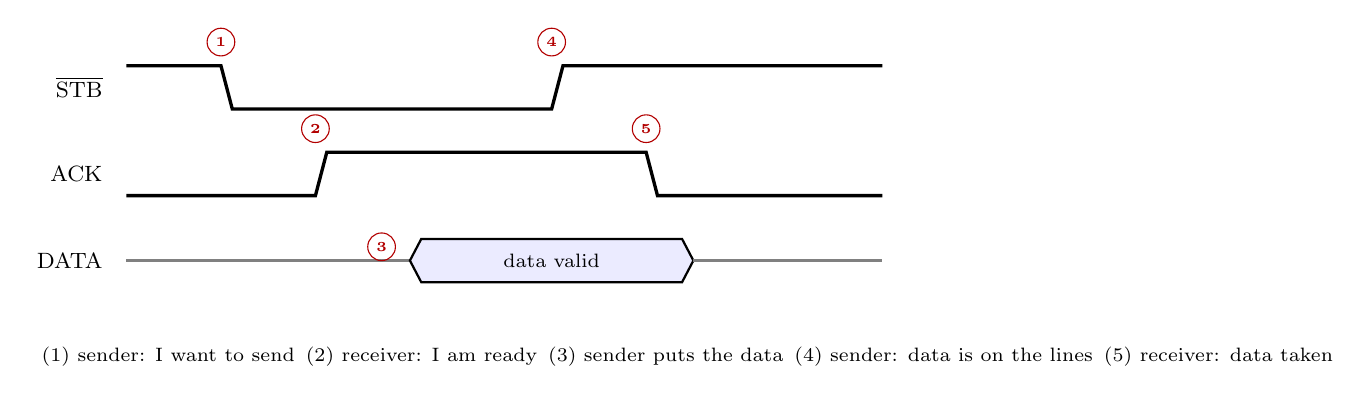
\begin{tikzpicture}[>=Stealth,font=\small,x=1.2cm,y=1cm]
% row 0 y=0
\node[anchor=east,font=\footnotesize,align=right] at (-0.15,0.275) {$\overline{\mathrm{STB}}$};
\draw[very thick] (0,0.55) -- (1,0.55) -- (1.12,0) -- (4.5,0) -- (4.62,0.55) -- (8,0.55);
% row 1 y=-1.1
\node[anchor=east,font=\footnotesize,align=right] at (-0.15,-0.825) {ACK};
\draw[very thick] (0,-1.1) -- (2,-1.1) -- (2.12,-0.55) -- (5.5,-0.55) -- (5.62,-1.1) -- (8,-1.1);
% row 2 y=-2.2
\node[anchor=east,font=\footnotesize,align=right] at (-0.15,-1.925) {DATA};
\draw[thick,gray] (0,-1.925) -- (3,-1.925);
\draw[thick,fill=blue!8] (3,-1.925) -- (3.12,-1.65) -- (5.88,-1.65) -- (6,-1.925) -- (5.88,-2.2) -- (3.12,-2.2) -- cycle;
\node[font=\scriptsize] at (4.5,-1.925) {data valid};
\draw[thick,gray] (6,-1.925) -- (8,-1.925);
\tikzset{n/.style={circle,draw=red!70!black,font=\tiny\bfseries,text=red!70!black,inner sep=0.5pt,minimum size=10pt}}
\node[n] at (1.0,0.85) {1};\node[n] at (2.0,-0.25) {2};\node[n] at (2.7,-1.75) {3};\node[n] at (4.5,0.85) {4};\node[n] at (5.5,-0.25) {5};
\node[font=\scriptsize,anchor=north west,align=left] at (-1.0,-2.9) {(1) sender: I want to send\enspace (2) receiver: I am ready\enspace (3) sender puts the data\enspace (4) sender: data is on the lines\enspace (5) receiver: data taken};
\end{tikzpicture}
\end{document}
